\section{Protection of nuclear DNA by lifespan-extending compounds in the yeast Saccharomyces cerevisiae}

\subsection{Нормальное название}

Защита ядерной ДНК с помощью веществ увеличивающих продолжительность жизни дрожжей Saccharomyces cerevisiae

\subsection{Абстракт}

АБСТРАКТ ГРАФИЧЕСКИЙ БЛЯТЬ

\begin{figure}[H]
	\centering
	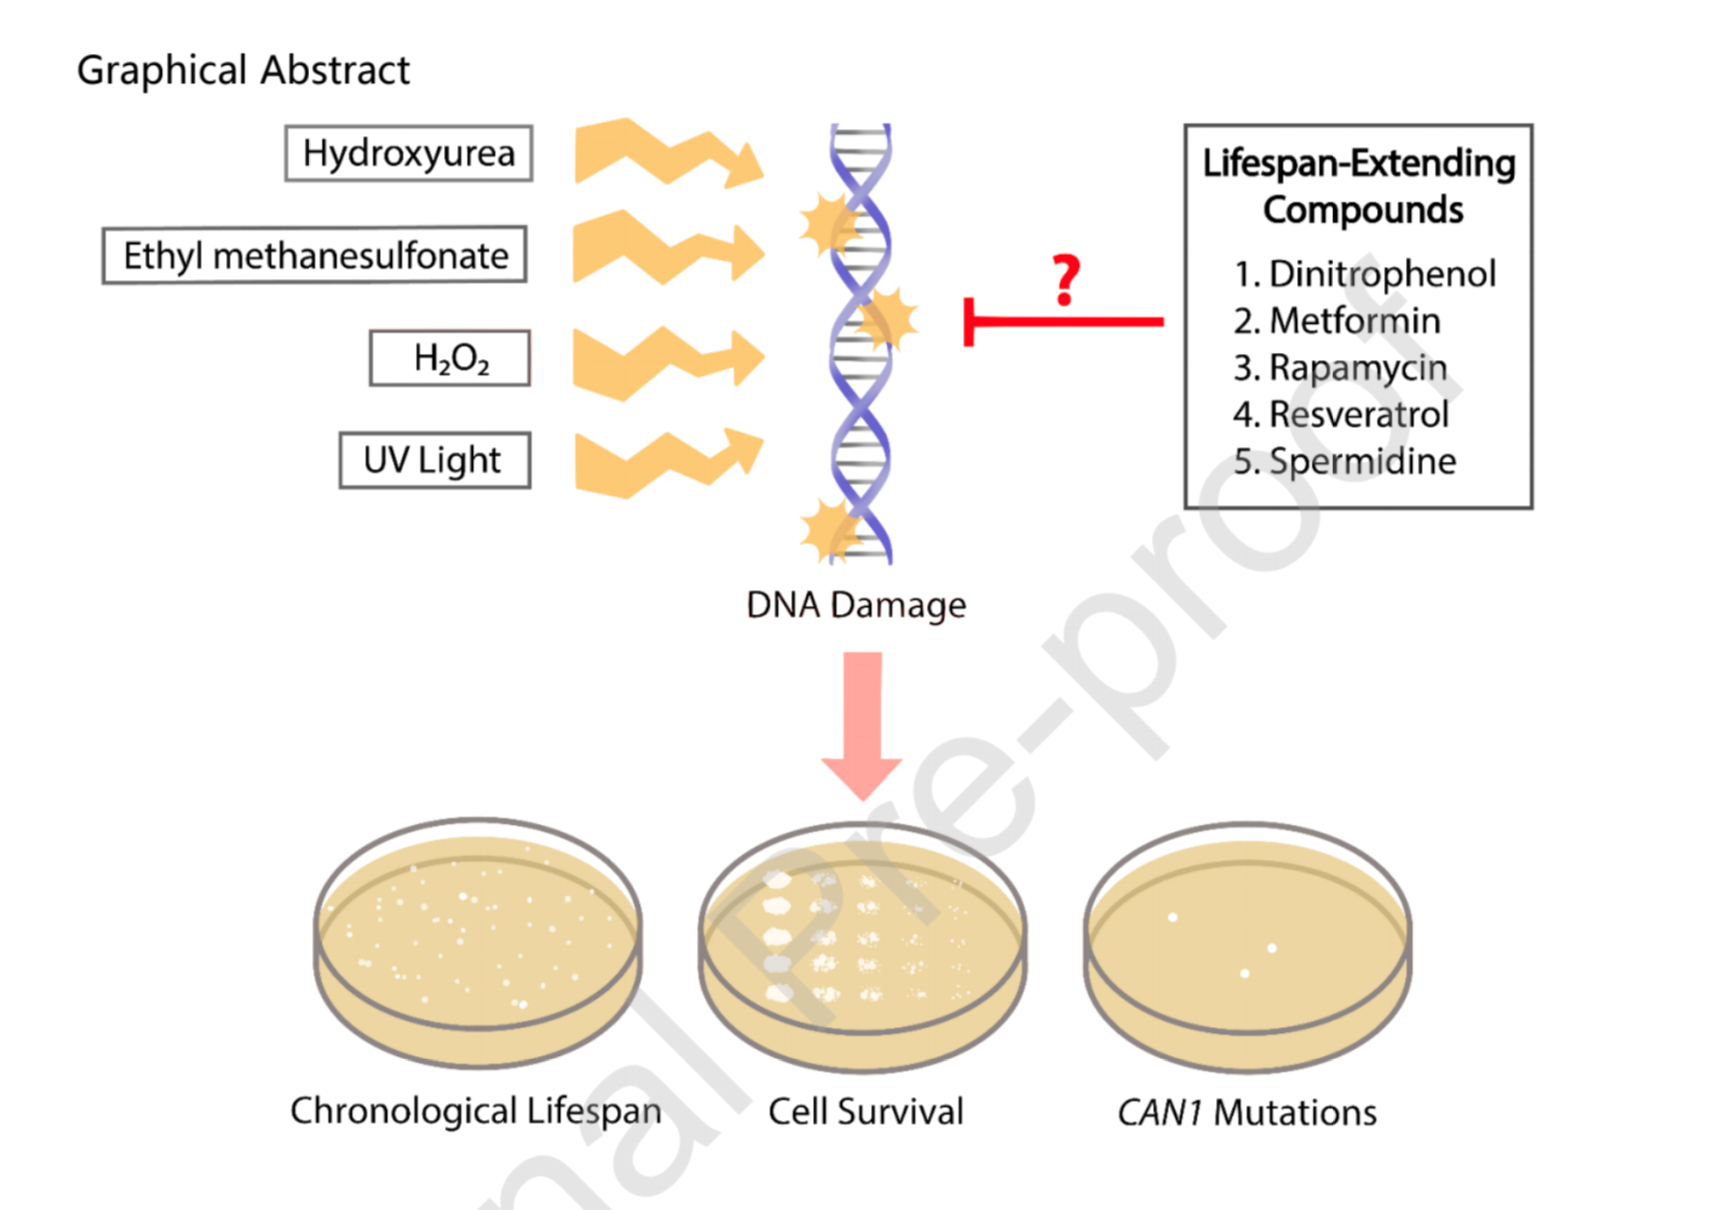
\includegraphics[width=\linewidth]{13_1}
	\caption{Графический абстракт: воздействие гидроксимочевины, этил метанасульфоната, перекиси водорода и УФ излучения приводят к повреждению ДНК. Продлевающие жизнь вещества. Три интересующих исследователей аспекта: продолжительность жизни, выживание клеток и мутации в фокусе CAN1}
\end{figure}

1.	Предположение-повреждение ДНК является причиной старения
2.	Существуют вещества, которые увеличивают продолжительность жизни модельных организмов (дрожжи, черви, мухи и мыши)
3.	Возможный механизм действия этих веществ-защита ДНК
4.	Исследовались 5 веществ: динитрофенол, метформин, рапамицин, ресвератрол и спермидин на возможность защиты ДНК (использовали дозы, которые показали эффективность в увеличении продолжительности жизни)
ЧТО ДЕЛАЛИ И ЧТО ПОЛУЧИЛИ?
5.	Рапамицин и спермидин снижают спонтанные мутации в локусе (месте) CAN1
6.	Динитрофенол, метформин и ресвератрол защищают от индуцированных этилметансульфанатом (EMS) мутаций CAN1 
7.	Все 5 защищают от EMS
8.	Метформин и спермидин защищают от УФ-излучения
9.	Все 5 не эффективны против H2O2 (перекись), спермедин только повысил эффект 
10.	Спермидин показал положительное действие против задержки роста гидроксимочивиной 
11.	ИТОГ: соединения увеличивающие продолжительность жизни могут частично защищать ядерную ДНК


\subsection{Картинки}

\begin{figure}[H]
	\centering
	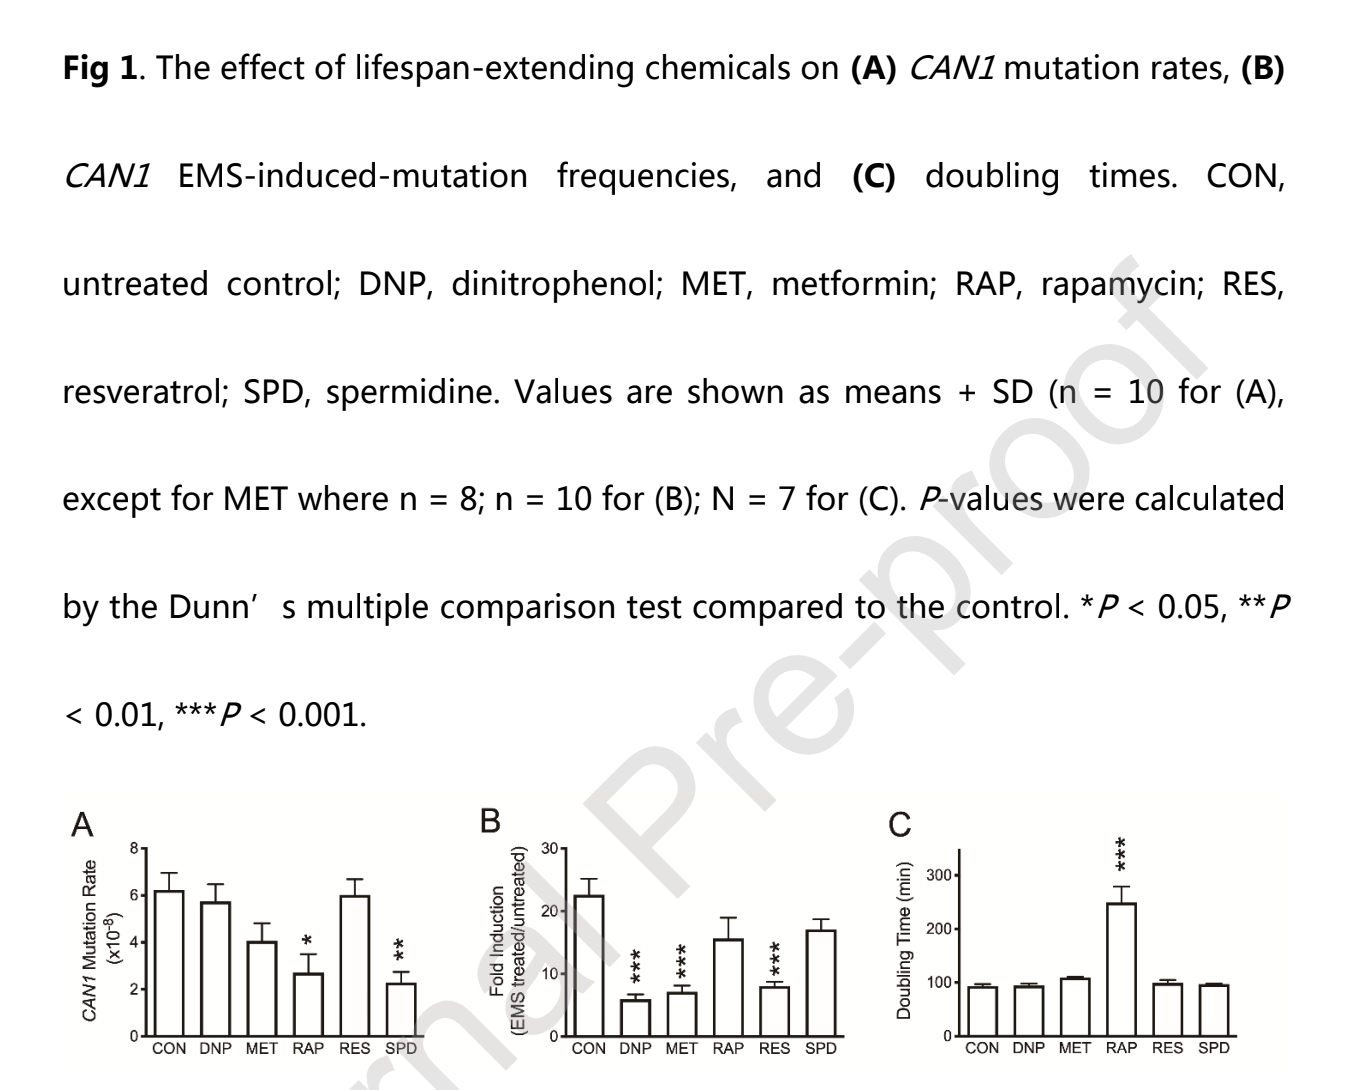
\includegraphics[width=\linewidth]{13_2}
	\caption{\textbf{A)}	Изменение темпа спонтанных (без внешних факторов) мутации в локусе CAN1 (CAN-канаванин) при воздействии: CON-контроль, ничего; DNP-динитрофенол; MET-метформин; RAP-рапамицин; RES-ресвератрол; SPD-спермидин; Показано, что RAP и SPD уменьшили в 1 и 2 раза соответственно.
		\textbf{B)}	Изменение темпа индуцированных (под воздействием метансульфонада) мутации в локусе CAN1 (CAN-канаванин) при воздействии: CON-контроль, ничего; DNP-динитрофенол; MET-метформин; RAP-рапамицин; RES-ресвератрол; SPD-спермидин; Показано, что  DNP, RES и MET в 3 раза уменьшили.
		\textbf{C)}	Изменение времени деления при воздействии: CON-контроль, ничего; DNP-динитрофенол; MET-метформин; RAP-рапамицин; RES-ресвератрол; SPD-спермидин; RAP замедляет в 3 раза
	}
\end{figure}

\begin{figure}[H]
	\centering
	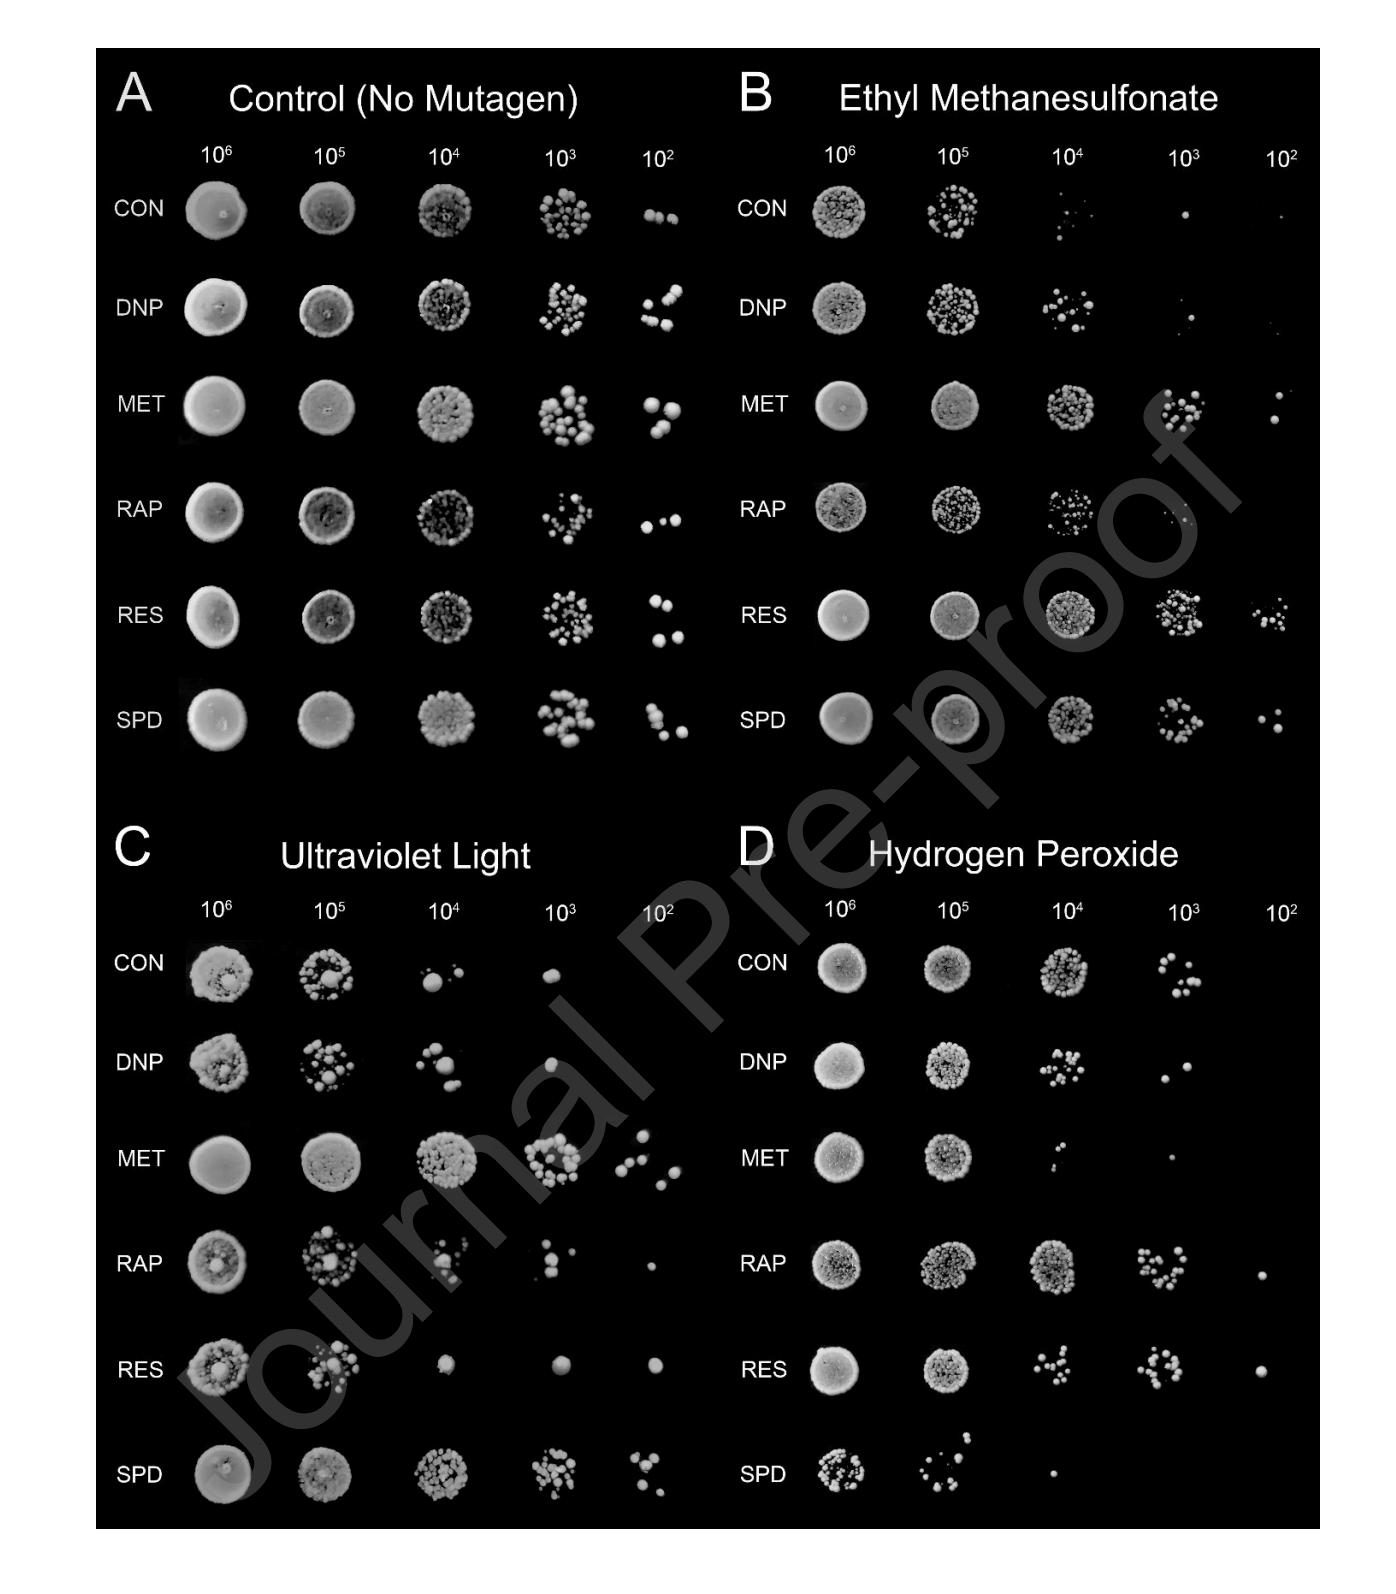
\includegraphics[width=\linewidth]{13_3}
	\caption{На рисунке изображены 4 панели для изучения вляния на колонии клеток \textbf{А-контроль}; \textbf{B-этилметансульфонат}; \textbf{С-УФ}; \textbf{D-перекись водорода}. Выращенные клетки воздействовали и делали последовательные разведения: DNP, dinitriphenol; MET, metformin; RAP, rapamycin; RES, resveratrol; SPD, spermidine.
	\textbf{B)} Выживание клеток без всего менее 1\% при введение веществ титры живых клеток увеличили
	\textbf{С)} Метформин и спермидин защищают от УФ-излучения
	\textbf{D)} Все 5 не эффективны против H2O2 (перекись), спермедин только повысил эффект 
}
\end{figure}


\begin{figure}[H]
	\centering
	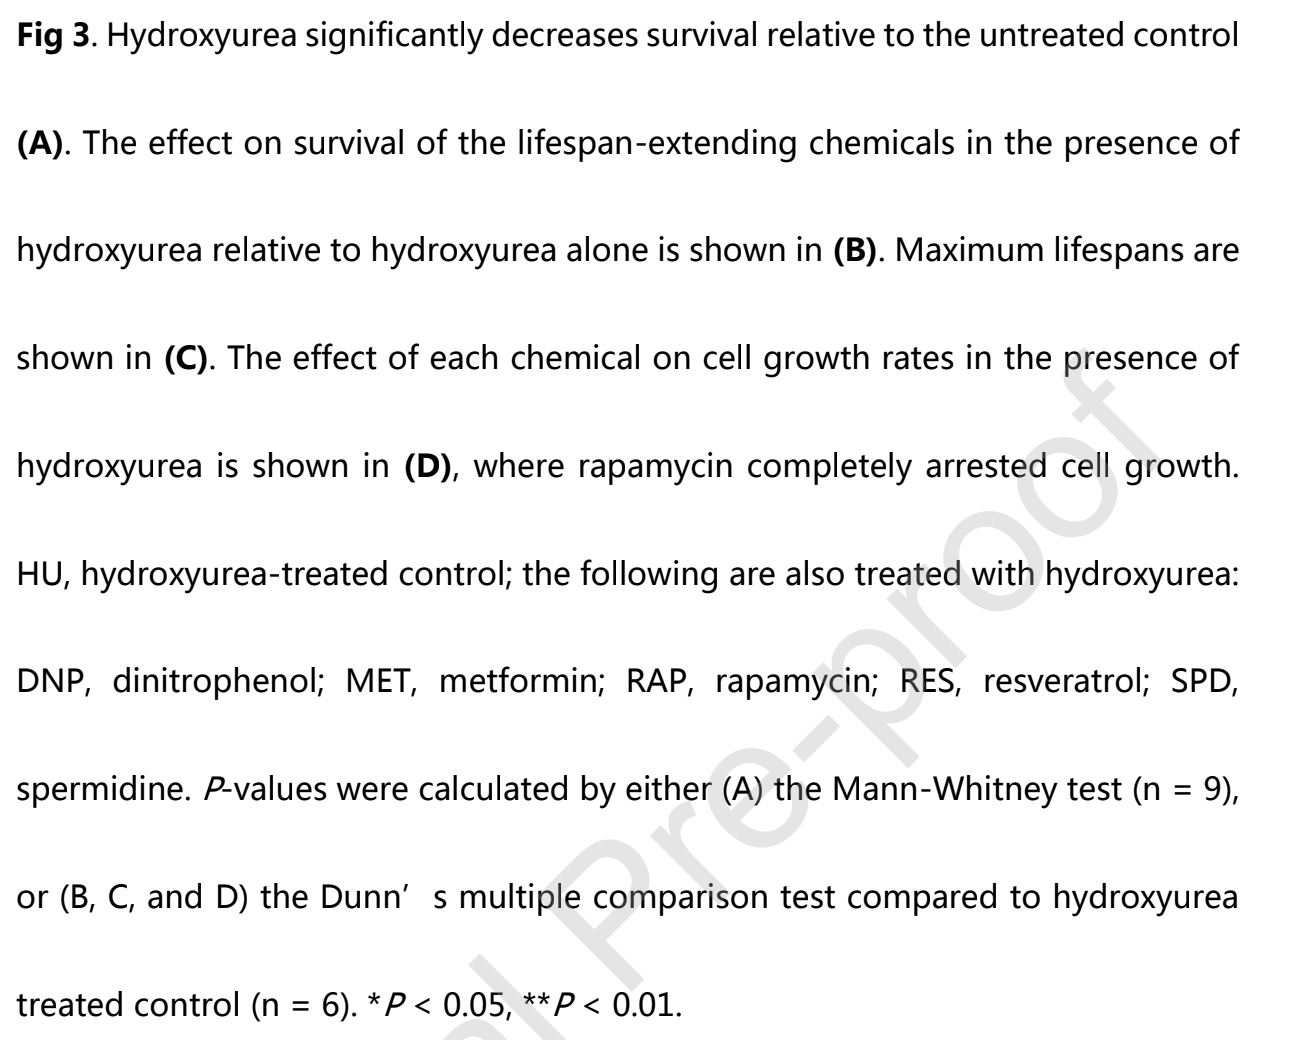
\includegraphics[width=\linewidth]{13_4}
	\caption{Провели эксперимент-вырастили в жидкой среде клетки и смотрят сколько дней протянут без добавления питательных веществ:
		\textbf{A)}	Процент выживаемости в зависимости от времени при пустой среде и при добавлении гидроксимочевины
		\textbf{B)} То же самое, но с добавлением продлевающих жизнь веществ. Видно, что эффект от спермедина лучше в примерно 10 раз в отличи от других.
	\textbf{C)}	Средняя продолжительность жизни по популяции, спермедин эффективен
	\textbf{D)}	Скорость роста в присутвии гидроксимочевиной. HU-контроль обработанный гидроксимочевиной, видно, что RAP полностью остановил рост клеток.
}
\end{figure}


\begin{figure}[H]
	\centering
		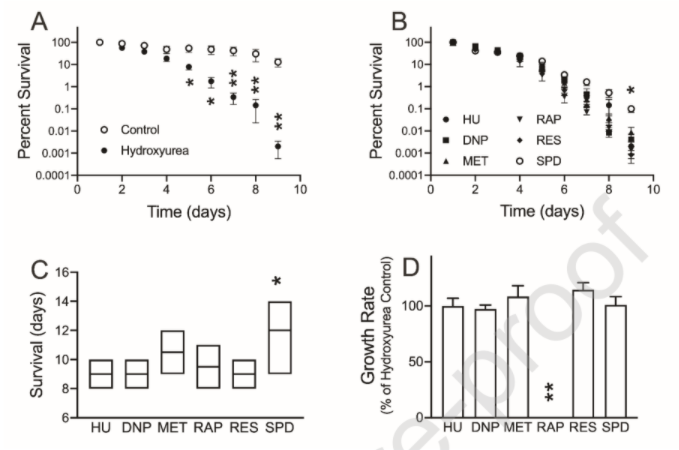
\includegraphics[width=\linewidth]{13.4.png}
		\caption{(\textbf{A}) Выживаемость дрожжей в присутствии гидроксикарбамида и без него. Далее все опыты в его присутствии. (\textbf{B}) Выживаемость при добавлений растворов исследуемых соединений. В обоих опытах A и B, видимо, декстроза добавлялась в течение опытов одинаковыми дозами таким образом, чтобы в контрольной группе выживаемость держалась на 100$\%$. По сравнению с контрольной группой, в растворе гидроксикарбамида выживаемость падает до $10^{-5}$. Из наших веществ только SPD повышает выживаемость в её присутствии - примерно на 2 порядка. (\textbf{C}) Среднее максимальное время жизни: в растворе SPD время жизни увеличивается на 2-3 дня в сравнении с растворами остальных веществ. (\textbf{D}) Относительная скорость роста (деления клеток) в присутствии гидроксикарбамида: (сравни с (\textbf{C})  первого графика) RAP полностью выключает рост.}
\end{figure}